\section{Results}
\label{sec:results}

\subsection{Coverage of the Saved Evidence}
The repository contains \CovGemini{} validated Gemini 3.5 Flash-Lite responses (\CovPct\% of the \NPromptsPerModel{} planned for that model). All of them reached the service's \texttt{STOP} finish reason with non-empty text, and they form \NPairs{} complete FLORES-200 translation pairs, \NPilotOverlap{} of which overlap the pilot set. No responses are yet saved for Qwen~2.5~1.5B (\CovQwen), Gemma~3 (\CovGemma) or NLLB-200 (\CovNLLB), and none for Gemini on KazParC, Belebele or the probes. All results below therefore concern Gemini translation on FLORES-200 unless stated otherwise; Table~\ref{tab:main} keeps the pending conditions visible.

\subsection{Main Translation Result}
Table~\ref{tab:main} and Fig.~\ref{fig:direction} report corpus scores. Gemini scored \GemChrfKK{} chrF2 (95\% CI $[\GemChrfKKLo, \GemChrfKKHi]$) when translating into Kazakh and \GemChrfEN{} ($[\GemChrfENLo, \GemChrfENHi]$) when translating into English. The directional gap was $\gap_{\mathrm{chrF2}} = \GemChrfGap$ points with a paired bootstrap interval of $[\GemChrfGapLo, \GemChrfGapHi]$, which excludes zero; relative to the English direction, the Kazakh score was \GemRelGapPct\% lower. BLEU showed the same ordering with a larger relative difference (\GemBleuKK{} vs.\ \GemBleuEN{}, $\gap = \GemBleuGap$). Both directions were far above the dictionary baseline (\DictChrfKK{} and \DictChrfEN{} chrF2), confirming that the outputs carry translation content rather than copied source text. The dictionary baseline itself showed a small gap in the opposite direction ($+\DictChrfGap$), which illustrates that directional differences are not guaranteed by the metric alone.

\begin{table*}[!t]
\centering
\caption{Translation Quality on \NPairs{} Paired FLORES-200 Items. Corpus Scores With 95\% Paired Bootstrap Intervals; Gap = EN$\rightarrow$KK Minus KK$\rightarrow$EN (Negative = Lower Quality Into Kazakh). Pending Systems Have No Saved Outputs Yet.}
\label{tab:main}
\small
\begin{tabular}{@{}lccc@{}}
\toprule
System & EN$\rightarrow$KK & KK$\rightarrow$EN & Gap (KK$-$EN) \\
\midrule
\multicolumn{4}{@{}l}{\textit{chrF2 $\uparrow$}} \\
Gemini 3.5 Flash-Lite & 56.40 {\scriptsize[54.11, 58.68]} & 65.33 {\scriptsize[63.13, 67.58]} & $-$8.93 {\scriptsize[$-$12.19, $-$5.64]} \\
Dictionary baseline & 2.48 {\scriptsize[2.05, 2.96]} & 1.70 {\scriptsize[1.36, 2.15]} & +0.78 {\scriptsize[0.44, 1.15]} \\
Qwen 2.5 1.5B & \multicolumn{3}{c}{\textit{pending (0 responses saved)}} \\
Gemma 3 & \multicolumn{3}{c}{\textit{pending (0 responses saved)}} \\
NLLB$-$200 600M & \multicolumn{3}{c}{\textit{pending (0 responses saved)}} \\
\multicolumn{4}{@{}l}{\textit{BLEU $\uparrow$}} \\
Gemini 3.5 Flash-Lite & 20.86 {\scriptsize[18.40, 23.42]} & 38.70 {\scriptsize[35.38, 42.00]} & $-$17.84 {\scriptsize[$-$21.83, $-$13.84]} \\
Dictionary baseline & 0.93 {\scriptsize[0.24, 1.72]} & 0.83 {\scriptsize[0.20, 1.54]} & +0.11 {\scriptsize[0.03, 0.19]} \\
Qwen 2.5 1.5B & \multicolumn{3}{c}{\textit{pending (0 responses saved)}} \\
Gemma 3 & \multicolumn{3}{c}{\textit{pending (0 responses saved)}} \\
NLLB$-$200 600M & \multicolumn{3}{c}{\textit{pending (0 responses saved)}} \\
\bottomrule
\end{tabular}

\end{table*}

\begin{figure}[!t]
\centering
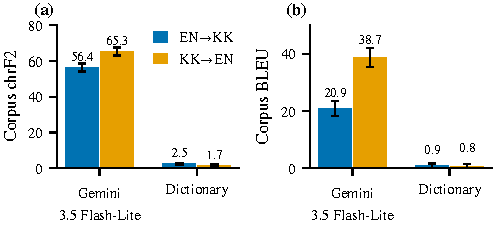
\includegraphics[width=\columnwidth]{figures/fig_direction.pdf}
\caption{Corpus (a) chrF2 and (b) BLEU by translation direction on the same \NPairs{} FLORES-200 items. Error bars are 95\% paired bootstrap intervals (\NBoot{} resamples, seed 42).}
\label{fig:direction}
\end{figure}

\subsection{Item-Level Evidence}
The corpus gap is not driven by a few items. Translation into Kazakh scored lower on \ItemsBelow{} of \NPairs{} items (\ItemsBelowPct\%; Fig.~\ref{fig:paired}a), and the median per-item difference was $\WilMed$ chrF2 points (Fig.~\ref{fig:paired}b). The Wilcoxon signed-rank test rejected equality of the paired sentence scores ($W=\WilW$, $p_{\mathrm{Holm}}=\WilP$) with a medium-to-large effect ($r_{\mathrm{rb}}=\WilR$; Table~\ref{tab:tests}). The two comparisons against the dictionary baseline were also significant in both directions. Item-level variation is nevertheless large: some items scored higher into Kazakh, and the three outputs written mainly in Latin script appear as clear outliers near zero.

\begin{figure}[!t]
\centering
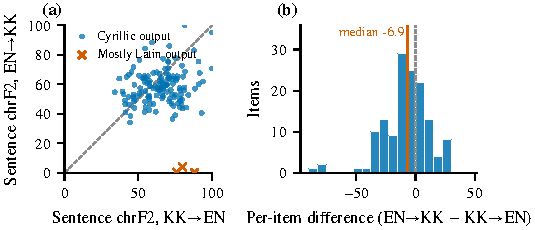
\includegraphics[width=\columnwidth]{figures/fig_paired.pdf}
\caption{(a) Sentence-level chrF2 of each item in both directions; points below the diagonal scored lower into Kazakh, and crosses mark outputs written mainly in Latin script. (b) Distribution of per-item differences; the orange line marks the median.}
\label{fig:paired}
\end{figure}

\begin{table}[!t]
\centering
\caption{Wilcoxon Signed-Rank Tests on Paired Sentence chrF2 ($n=\NPairs$). $\Delta$ Follows the Order Shown; $r_{\mathrm{rb}}$ Is the Matched-Pairs Rank-Biserial Correlation.}
\label{tab:tests}
\footnotesize
\resizebox{\columnwidth}{!}{\begin{tabular}{@{}lrrrr@{}}
\toprule
Comparison & Median $\Delta$ & $W$ & $p_{\mathrm{Holm}}$ & $r_{\mathrm{rb}}$ \\
\midrule
Gemini: EN$\rightarrow$KK vs.\ KK$\rightarrow$EN & -6.90 & 2564 & $2.1\times10^{-6}$ & -0.47 \\
Gemini vs.\ dictionary, EN$\rightarrow$KK & +54.62 & 3 & $6.5\times10^{-24}$ & +1.00 \\
Gemini vs.\ dictionary, KK$\rightarrow$EN & +64.38 & 0 & $6.5\times10^{-24}$ & +1.00 \\
\bottomrule
\end{tabular}
}
\end{table}

\subsection{Robustness and Sensitivity}
Table~\ref{tab:robust} and Fig.~\ref{fig:forest} show that the direction of the gap does not depend on the metric or on the analysed subset. chrF++ ($\GemChrfPPGap$), BLEU ($\GemBleuGap$) and TER ($+\GemTerGap$, where higher is worse) all indicate lower quality into Kazakh, and all four intervals exclude zero. Removing the \NPilotOverlap{} items that overlap the pilot set changed the chrF2 gap by less than 0.03 points ($\GapNoPilot$, $[\GapNoPilotLo, \GapNoPilotHi]$). Removing the \NMostlyLatin{} mostly Latin-script outputs reduced the gap to $\GapNoLatin$ ($[\GapNoLatinLo, \GapNoLatinHi]$), so script errors explain part, but clearly not most, of the difference. The gap was negative in all three FLORES domains and in all three source-length groups; the interval for short sources (up to \LenCutLo{} words) included zero. These subgroup estimates are exploratory and their intervals overlap. Source length was only weakly associated with sentence chrF2 (Spearman $\rho=\RhoLenKK$ into Kazakh, $\RhoLenEN$ into English).

\begin{table}[!t]
\centering
\caption{Robustness of the Directional Gap. Gaps With 95\% Paired Bootstrap Intervals. $^{\dagger}$For TER, Lower Is Better, so a Positive Gap Indicates Lower Quality Into Kazakh.}
\label{tab:robust}
\footnotesize
\begin{tabular}{@{}lrcc@{}}
\toprule
Analysis & $n$ & Gap & 95\% CI \\
\midrule
\multicolumn{4}{@{}l}{\textit{Metric (all pairs)}} \\
chrF2 (primary) & 138 & $-$8.93 & [$-$12.19, $-$5.64] \\
chrF++ & 138 & $-$11.28 & [$-$14.50, $-$7.92] \\
BLEU & 138 & $-$17.84 & [$-$21.83, $-$13.84] \\
TER$^{\dagger}$ & 138 & +18.55 & [13.93, 23.02] \\
\multicolumn{4}{@{}l}{\textit{Sensitivity (chrF2)}} \\
Pilot items removed & 124 & $-$8.91 & [$-$12.51, $-$5.48] \\
Latin-script outputs removed & 135 & $-$7.28 & [$-$10.00, $-$4.27] \\
\multicolumn{4}{@{}l}{\textit{Subgroup (chrF2, exploratory)}} \\
Domain: wikibooks & 49 & $-$6.50 & [$-$10.19, $-$2.50] \\
Domain: wikinews & 46 & $-$12.39 & [$-$18.39, $-$6.42] \\
Domain: wikivoyage & 43 & $-$7.83 & [$-$14.83, $-$1.69] \\
Length: short & 48 & $-$4.37 & [$-$10.14, 1.14] \\
Length: medium & 46 & $-$13.89 & [$-$19.60, $-$8.19] \\
Length: long & 44 & $-$7.76 & [$-$13.02, $-$3.44] \\
\bottomrule
\end{tabular}

\end{table}

\begin{figure}[!t]
\centering
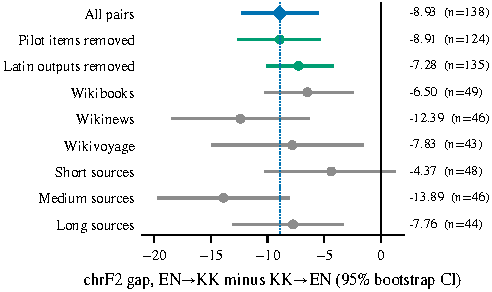
\includegraphics[width=\columnwidth]{figures/fig_forest.pdf}
\caption{chrF2 gap (EN$\rightarrow$KK minus KK$\rightarrow$EN) with 95\% bootstrap intervals for all pairs (blue), the planned sensitivity analyses (green) and exploratory subgroups (grey). The dotted line marks the overall estimate.}
\label{fig:forest}
\end{figure}

\subsection{Diagnostic 1: Script}
Of the \NPairs{} Kazakh outputs, \NMostlyLatin{} were written mainly in Latin-script Kazakh and \NAnyLatin{} contained at least one Latin letter. Latin letters are not errors in themselves: \NRefLatin{} of the professional Kazakh references also contain Latin characters, typically names, units or abbreviations such as ``pH''. The mostly Latin outputs, however, score near zero chrF2 against Cyrillic references even when parts of them are readable, because character n-grams cannot match across scripts.

\subsection{Diagnostic 2: Inflection-Tolerant Matching}
Exact word recall against the reference was much lower for Kazakh outputs (\RecallKK\%) than for English outputs (\RecallEN\%). Fig.~\ref{fig:inflection} shows how many additional reference words are matched when words are compared by their first $k$ letters. At $k=\KPrimary$, \NmKK\% of Kazakh reference words (95\% CI $[\NmKKLo, \NmKKHi]$) were matched only at the prefix level, compared with \NmEN\% ($[\NmENLo, \NmENHi]$) of English ones, a difference of \NmDiff{} percentage points ($[\NmDiffLo, \NmDiffHi]$). The mismatched-reference control produced only \NmCtrlKK\% and \NmCtrlEN\%, so chance prefix collisions do not explain the pattern. Put differently, about \NmShareOfMissKK\% of the Kazakh reference words that the model did not reproduce exactly appeared in the output with the same five-letter beginning but a different ending, against \NmShareOfMissEN\% in English. The Kazakh excess was present at every prefix length from 3 to 8.

\begin{figure}[!t]
\centering
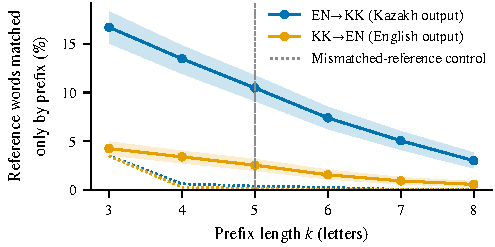
\includegraphics[width=\columnwidth]{figures/fig_inflection.pdf}
\caption{Share of reference words matched only after both texts are cut to $k$-letter prefixes (same beginning, different ending), with 95\% bootstrap bands. Dotted lines show the mismatched-reference control. The dashed vertical line marks the main setting $k=\KPrimary$.}
\label{fig:inflection}
\end{figure}

Table~\ref{tab:ablation} reports the corresponding ablation. Cutting all words to five letters shrank the BLEU gap from $\AblBleuGapFull$ to $\AblBleuGapK$ (\AblBleuRedPct\% smaller) and the word-F1 gap from $\AblFoneGapFull$ to $\AblFoneGapK$ (\AblFoneRedPct\% smaller), whereas the chrF2 gap was essentially unchanged ($\AblChrfGapK$). Word-level metrics thus overstate the Kazakh deficit partly because they treat every suffix difference as a complete miss, while chrF2 already gives partial credit for shared stems. The substantial gap that remains after truncation indicates that differences beyond word endings---lexical choices, omissions, additions and reordering---also contribute.

\begin{table}[!t]
\centering
\caption{Ablation: Directional Gaps After Cutting Every Word in Outputs and References to Its First $k$ Letters ($n=\NPairs$).}
\label{tab:ablation}
\footnotesize
\begin{tabular}{@{}lccc@{}}
\toprule
Word form & chrF2 gap & BLEU gap & Word-F1 gap \\
\midrule
Full forms & -8.93 & -17.84 & -22.01 \\
6-letter prefix & -9.10 & -14.19 & -16.31 \\
5-letter prefix & -9.00 & -13.24 & -14.28 \\
4-letter prefix & -8.82 & -12.38 & -12.19 \\
\bottomrule
\end{tabular}

\end{table}

\subsection{Diagnostic 3: Token Usage}
For translations of the same \NPairs{} source sentences, Kazakh outputs consumed \TokRatio{} times as many output tokens as English outputs (95\% CI $[\TokRatioLo, \TokRatioHi]$), although they were only \CharRatio{} times as long in characters. Per character, Kazakh required \TokPerCharKK{} tokens per 100 characters against \TokPerCharEN{} for English, a premium of \TokCharPrem$\times$ ($[\TokCharPremLo, \TokCharPremHi]$; Fig.~\ref{fig:tokens}a). The input side gave a consistent estimate: regressing prompt tokens on source length in both directions yielded \TokSrcRatio{} times as many tokens per character for Kazakh sources. At the level of individual items, the token ratio was not associated with the chrF2 gap (Spearman $\rho=\RhoTok$, $p=\RhoTokP$; Fig.~\ref{fig:tokens}b). Tokenization therefore represents a consistent cost burden for Kazakh, but within this sample it does not predict which sentences are translated worse. Median request latency was \LatKK{}~s into Kazakh and \LatEN{}~s into English; because latency includes the public network path, we do not interpret it further.

\begin{figure}[!t]
\centering
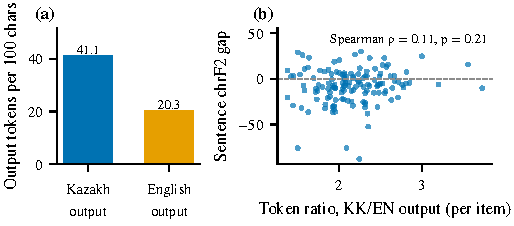
\includegraphics[width=\columnwidth]{figures/fig_tokens.pdf}
\caption{(a) Visible output tokens per 100 characters reported by the Gemini API for the same \NPairs{} items. (b) Per-item ratio of Kazakh to English output tokens against the per-item chrF2 gap.}
\label{fig:tokens}
\end{figure}

\subsection{Question Answering Calibration}
No model QA responses have been saved yet, so H1 for QA cannot be tested. Table~\ref{tab:qa} reports the two language-blind rules on all \NQa{} paired Belebele questions. Always answering~A scored \QaAKK\% in both languages. A single seeded random guesser scored \QaRndKK\% in Kazakh and \QaRndEN\% in English, with \QaRndKKonly{} items correct only in Kazakh and \QaRndENonly{} only in English (exact McNemar $p=\QaRndP$). An 8.5-point difference can therefore arise from a rule that uses no language information at all, which shows why paired tests on discordant items, rather than raw accuracy differences, are required for the model comparison.

\begin{table}[!t]
\centering
\caption{QA Accuracy on \NQa{} Paired Belebele Questions With Exact 95\% Intervals, Discordant Pairs and Exact McNemar $p$-Values}
\label{tab:qa}
\footnotesize
\resizebox{\columnwidth}{!}{\begin{tabular}{@{}lccrr@{}}
\toprule
Condition & Kazakh (\%) & English (\%) & KK/EN only & $p$ \\
\midrule
Always A & 19.5 {\scriptsize[14.2, 25.7]} & 19.5 {\scriptsize[14.2, 25.7]} & 0/0 & 1.000 \\
Seeded random & 18.5 {\scriptsize[13.4, 24.6]} & 27.0 {\scriptsize[21.0, 33.7]} & 29/46 & 0.064 \\
Gemini 3.5 Flash-Lite & \multicolumn{4}{c}{\textit{pending: no QA responses saved}} \\
Qwen 2.5 1.5B & \multicolumn{4}{c}{\textit{pending: no QA responses saved}} \\
Gemma 3 & \multicolumn{4}{c}{\textit{pending: no QA responses saved}} \\
\bottomrule
\end{tabular}
}
\end{table}

\subsection{Qualitative Review of Low-Scoring Outputs}
To illustrate what the scores penalise, the \NReviewed{} Kazakh outputs with the lowest sentence chrF2 received provisional labels in an AI-assisted first pass that the authors reviewed against the source and the output (Table~\ref{tab:labels}). This is a single, unblinded pass on a sample selected for low scores, so its proportions describe the tail and not Kazakh output in general, and it does not substitute for the planned blind annotation. The most frequent outcome (\LabReferenceMismatch{} of \NReviewed) was a plausible translation phrased differently from the single reference, which confirms that low chrF2 does not always mean a wrong translation. Lexical problems (\LabLexical) included non-words such as \kk{беінші}{beinshi} for \kk{бесінші}{besinshi} (``fifteenth'') and Russian spellings such as \kk{Цыган}{Tsygan} for Kazakh \kk{Сыған}{Syghan}. Semantic problems (\LabSemantic) included rendering ``worked to death'' as ``tortured to death''. The \LabScript{} script cases were whole sentences in Latin-script Kazakh. Only \LabMorphological{} case was labelled primarily morphological (\kk{әрпи}{ärpiy} instead of the possessive form \kk{әрпі}{ärpi}); because each case received a single primary label, suffix errors that co-occur with lexical problems are not counted separately.

\begin{table}[!t]
\centering
\caption{First-Pass Labels of the \NReviewed{} Lowest-chrF2 EN$\rightarrow$KK Outputs (Provisional AI-Assisted Pass Reviewed by the Authors; Blind Double Annotation Pending)}
\label{tab:labels}
\footnotesize
\begin{tabular}{@{}lrr@{}}
\toprule
First-pass label & Count & Share (\%) \\
\midrule
Reference mismatch & 13 & 43.3 \\
Lexical & 9 & 30.0 \\
Semantic & 4 & 13.3 \\
Script & 3 & 10.0 \\
Morphological & 1 & 3.3 \\
\midrule
Total & 30 & 100.0 \\
\bottomrule
\end{tabular}

\end{table}
